%%%%%%%%%%%%%%%%%%%%%%%%%%%%%%%%%%%%%%%%%%%%%%%%%%%
%
%  New template code for TAMU Theses and Dissertations starting Fall 2016.
%
%  Author: Sean Zachary Roberson
%	 Version 3.16.09
%  Last updated 9/12/2016
%
%%%%%%%%%%%%%%%%%%%%%%%%%%%%%%%%%%%%%%%%%%%%%%%%%%%

%%%%%%%%%%%%%%%%%%%%%%%%%%%%%%%%%%%%%%%%%%%%%%%%%%%%%%%%%%%%%%%%%%%%%%%
%%%                           SECTION II
%%%%%%%%%%%%%%%%%%%%%%%%%%%%%%%%%%%%%%%%%%%%%%%%%%%%%%%%%%%%%%%%%%%%%%


\chapter{PRELIMINARY RESULTS AND CURRENT EFFORTS}
Our preliminary results consist of an evaluation of pixel distribution distances as an effective metric, as well as the exploration of other image features to be used in our learning algorithm.
In our prelimiary analysis we had access to a small dataset; we have recently gained access to a much larger dataset which we are currently cleaning and labeling in order to further our training and analysis.
This analysis was performed on greyscale images, as we did not yet have access to images with many bands, and greyscale or average intensity values have traditionally proven to be effective for image analysis.

\section{Image feature evaluation}
In this problem, we wish to find a set of features which can be quickly extracted from images, and used to train a model to identify images that do not belong in the stream.
The first step in this process is to evaluate features to find ones that are suitable to our needs: quickly extracted and distinguishing between overlapping and non-overlapping images.

When thinking of the differences between overlapping and non-overlapping images, pixel distribution was one of our first ideas.
Pixel distribution is a very simple feature to extract: it can be done in linear time with respect to the number of pixels, and is easily distributable.
Furthermore, it is clear that images with a large overlap will have fairly similar pixel distributions (since much of their conent is identical), and non-overlapping images may not.


\subsection{Distribution Distances}

Once pixel distributions are extracted, a method for comparing the distributions is needed.
From the field of statistics, there are a few methods for calculating \"distances\" between distributions: the higher the distance, the less similar the distributions are in some way.

The first distance metric we looked at is a very common method for calculating the distance between two sets of numbers: the mean-squared error or MSE.
Essentially, the MSE is the L-2 norm of the errors or differences between the two sets of numbers.
If we consider the first distribution to be the vector $\underline{\mathbf{p}}$ to be one distribution and the vector $\underline{\mathbf{q}}$ to be another distribution, each of length n, then the MSE is given by:
\begin{equation}
\frac{1}{n} \left( \sum_{i=1}^n{(p_i-q_i)^2} \right)^{1/2} .
\end{equation}

While the MSE does provide a distance between the two distributions, it is more suited to calculating errors, as the name suggests.
Another distance metric, called the Bhattacharyya distance, is actually designed to measure the similarity between two continuous or discrete probability distributions.
It is calculated by taking the negative of the log of the closely related Bhattacharyya coefficient.
The Bhattacharyya coefficient was designed to be a metric for the amount of overlap between two distributions, defined as:
\begin{equation}
BC(\mathbf{p}, \mathbf{q}) = \sum_{i=1}^n{\sqrt{p_iq_i}} .
\end{equation}
Making the Bhattacharyya distance equal to:
\begin{equation}
BD(\mathbf{p}, \mathbf{q}) = - \ln \left( \sum_{i=1}^n {\sqrt{p_iq_i}} \right) .
\end{equation}

Our results were predictably better using the Bhattacharyya distance rather than the MSE, so this distance metric was used for evaluation of distributions as a distinguishing feature.
It is worth noting that both of these distance metrics are caluclated in linear time with respect to the number of possible intensity values.


\subsection{Application to images with peak-finding}

In order to evaluate the effectiveness of the Bhattacharyya distance as a distinguishing feature, we calculated the distance between distributions of consecutive images in our datasets.
Even between the two flights contained in our dataset, the means and variances between flights were widely different, making a simple threshold invalid as a classifier.
Instead, we considered the distance values as a signal and used the peak-finding capabilities in SciPy to correlate spikes in the distances with the anomalous images we are trying to detect.

Below are two figures showing the distance metrics of our two flights with the detected peaks marked:

\begin{figure}[h]
\centering
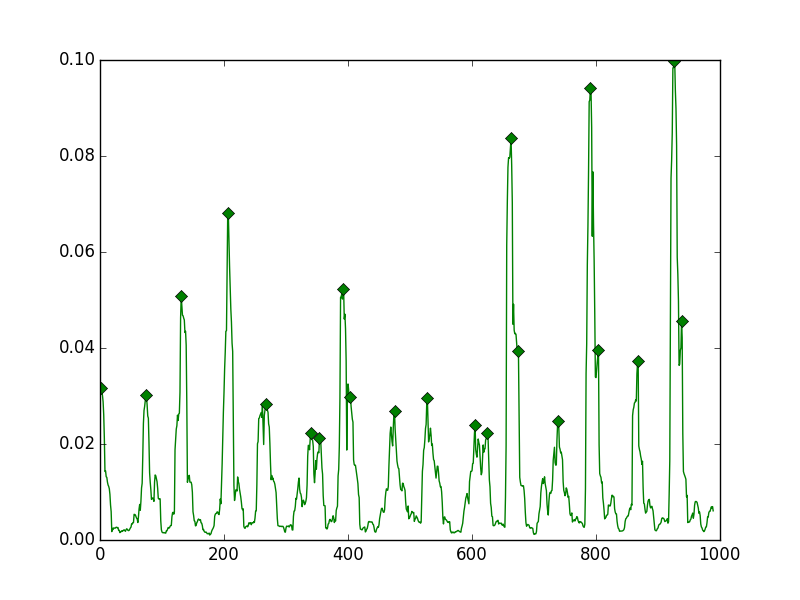
\includegraphics[scale=.50]{figures/608pf}
\caption{Plot of Bhattacharyya distances for the flight on 6/08/16}
\label{fig:tamu-fig1}
\end{figure}

\begin{figure}[h]
\centering
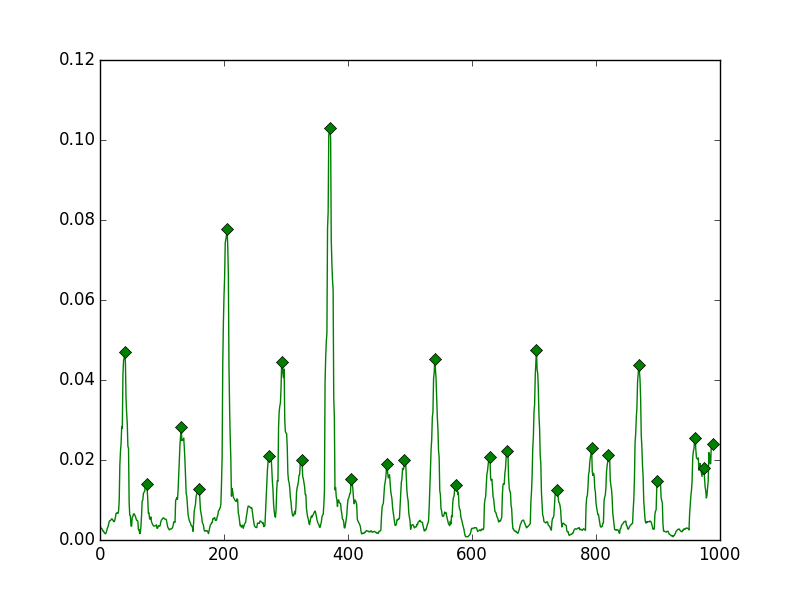
\includegraphics[scale=.50]{figures/629pf}
\caption{Plot of Bhattacharyya distances for the flight on 6/29/16}
\label{fig:tamu-fig2}
\end{figure}

Between both flight datasets, we achieved a detection rate of 66.0\% and a false alarm rate of 24.1\%.
While this is not an acceptable level of performance for the system as a whole, it is effective enough to be useful among a set of features used in a training algorithm.
One reason why this feature does not perform better is that it discards all spatial information in the images; any permutation of the pixels will result in the same pixel distribution.
Furthermore, this feature alone will perform poorly in distinguishing out-of-sync images that happen to be over a homogeneous area, as the pixel distributions will still be close.


\subsection{Other features}

As stated, other features are needed in order to create a robust detection system.
From the field of image processing, there are many image features that can be calculated quickly; our goal is to find features which can be compared and matched among consecutive images in a stream to determine if the images are overlapping by the desired amount.

From previous research into image classification using feature descriptiors \cite{anomalyhyper}, we have identified the SIFT feature as a potential feature which does incorporae spatial information.
This is a scale-invariant feature transform which can be implemented in real time.
Another potential feature with similar attributes is called CenSurE \cite{censure} , which we are also testing.
Other easily computable feature descriptors that we are considering include the BRIEF binary descriptor and the DAISY dense feature description.
The idea with these feature descriptors is to locate a set of keypoints in each image, and then attempt to match them between images to infer that the regions enclosed by matched descriptors are overlapping.

A different feature we are testing is the segmentation and classification of textures within each image using Local Binary Patterns (LBP).
Utilizing the percentage of an image occupied by certain image textures yields a feature similar to the pixel distribution, but over regions of the image rather than on an individual pixel level.
This idea extends naturally into using the multiple bands in multispectral or hyperspectral images for texture classification.


\section {Current efforts}
Our current efforts are split between data gathering and algorithm development.
As mentioned, we have recently gained access to a large amount of raw data for use in this project.
However, the data still needs to be cleaned and labeled before it can be used in algorithm development and assessment.

ALgorithm development has been focused on writing a framework in which we can assess the performance of different image features as well as detection algorithms.
Once the data is prepared, the above mentioned image features will be calculated and used as a feature vector to train and run various learning algorithms.


\subsection{Potential Learning Algorithms}

Among the many supervised learning classification algorithms, we have selected a few that we believe will perform this detection well.
The first among these is logistic regression: one of the most widely used classification algorithms.
Logistic regression takes a labeled training set of feature vectors $\mathbf{x^{(i)}}$ and corresponding binary labels $\mathbf{y^{(i)}}$.
It then finds $\theta$ to minimze the cost function:
\begin{equation}
J(\theta) = \frac{1}{m} \sum_{i=1}^m\frac{1}{2} \left( h_\theta \left( x^{(i)} \right) - y^{(i)} \right)^2
\end{equation}
where $h_\theta (\cdot)$ is the logistic function defined as $h_\theta(x) = \frac{1}{1+e^{-\theta^Tx}}$.

The next learning algorithm we have selected is the backpropagation artificial neural network (ANN).
An ANN is a highly connected directed graphical model, in which the nodes are separated into layers.
In the first layer, called the input layer, your observation or data is input into the layer's nodes.
From here, the information propagates from layer to layer according to the weights of the connections between nodes in each layer.
In training, the output at the final layer is compared to the desired output, and connection weights are adjusted according to the error.
ANNs have massive potential for performing at tasks which are difficult to define or explicity program, but often require a large amount of training data and time to become effective.
The typical neural network diagram is displayed below for clarity.

One of the other possible classification algorithms being considered is the decision tree. 
Since it operates much differently from the other algorithms being considered, the decision tree may prove useful as a point of comparsion.
A decision tree takes a labeled training set of feature vectors $\mathbf{x^{(i)}}$ and corresponding binary labels $\mathbf{y^{(i)}}$, and finds a set of ordered thresholds to compare the features to in order to classify the vector.
This can be visualized as a tree, in which you start at the root node, and move down the tree according to the thresholds defined at the nodes.
Leaf nodes contain the predicted classification.

By comparing the performance of these algorithms, along with the previously mentioned peak-finding, with the image features desired, we believe we can gain a better understanding of the performance of different learning algorithms for this problem, while simultaneously creating a useful system for our intended application.

\begin{figure}[h]
\centering
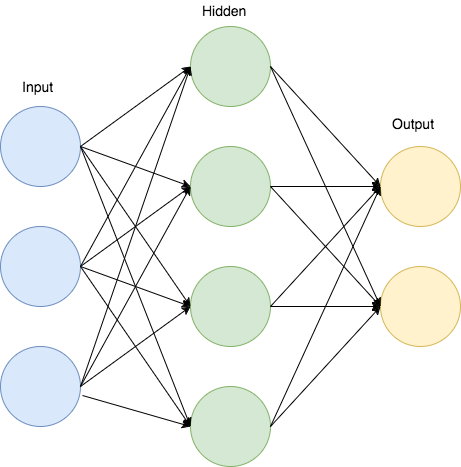
\includegraphics[scale=.50]{figures/NN}
\caption{A general ANN}
\label{fig:tamu-fig3}
\end{figure}



